\chapter{LFT: Lattice with Fermions}
We will now introduce Fermions on the lattice. Parts of this presentation 
follows Chapters 5 and 10 of~\cite{gattringer_quantum_2010}. 
We will start in the continuum
and introduce a naive discretization. Then we will go into detail, point
out a problem with the naive discretization, and fix it. We will omit
space-time dependence sometimes for the sake of brevity, but it should
be clear which objects have space-time dependence anyway. Primarily
we are interested in studying QCD, so $N_c=3$. This chapter uses Dirac
algebra extensively, but the algebra is different when the metric
is Euclidean. For details see \apref{ap:spec_math}.

In the continuum theory, the free fermion propagator is
\begin{equation}
  S_F=\int\dd[4]{x}\bar{\psi}(\slashed{\partial}+m)\psi.
\end{equation}
Using the rules~\eqref{eq:dertodiff} and \eqref{eq:inttosum}, one naively
discretizes this action on the lattice as
\begin{equation}\label{eq:naivefermact}
  S_F=a^4\sum_x\bar{\psi}(x)\left(\sum_{\mu=1}^4\gamma_\mu
       \frac{\psi(x+a\hat{\mu})-\psi(x-a\hat{\mu})}{2a}
       +m\psi(x)\right).
\end{equation}
The fermionic partition function is
\begin{equation}
  Z_F=\int\DD{\psi}\DD{\bar{\psi}}e^{-S_F},
\end{equation}
with integration measure
\begin{equation}
  \int\DD{\psi}\DD{\bar{\psi}}
   =\prod_{x,f,\alpha,c}\dd{\bar{\psi}^f_{\alpha c}(x)}
                        \dd{\psi^f_{\alpha c}(x)},
\end{equation}
where $f$ runs over flavors, $\alpha$ runs over Dirac indices, and $c$
runs over colors.

In addition, we want the fermionic action to be gauge invariant. The
gauge transformation for fermion fields
\begin{equation}
  \psi(x)\to U(x)\psi(x),~~~~~\bar{\psi}(x)\to\bar{\psi}(x)U(x)^\dagger
\end{equation}
with $U\in\SU(3)$ reminds us of the gauge transformation for scalar 
fields given in Chapter~\ref{ch:preliminaries}. Working in the continuum 
we introduce, just as before, a gauge field $A_\mu(x)$ so that the 
fermionic action becomes
\begin{equation}
  S_F=\int\dd[4]{x}\bar{\psi}\big(\gamma_\mu(\partial_\mu+A_\mu)+m\big)\psi.
\end{equation}
The gauge-transformed fermionic action is
\begin{equation}
  S'_F=\int\dd[4]{x}\bar{\psi}\,U^\dagger
        \big(\gamma_\mu(\partial_\mu+A'_\mu)+m\big)U\psi,
\end{equation}
so that the requirement of gauge invariance leads us to conclude
\begin{equation}
  (\partial_\mu+A_\mu)\psi=U^\dagger(\partial_\mu+A'_\mu)U\psi.
\end{equation}
Solving for $A'_\mu$ we find
\begin{equation}
  A'_\mu=(\partial_\mu U)U^\dagger-UA_\mu U^\dagger,
\end{equation}
just as we did before.

On the lattice, link variables transform as
\begin{equation}
  U_\mu(x)\to U'_\mu(x)=U(x)U_\mu(x)U^\dagger(x+a\hat{\mu}),
\end{equation}
which ensures that closed loops of link variables are gauge invariant.
In addition the discretized fermionic action becomes gauge invariant
when it is written as
\begin{equation}\label{eq:naivefermactgauge}
  S_F=a^4\sum_x\bar{\psi}(x)\left(\sum_{\mu=1}^4\gamma_\mu
       \frac{U_\mu(x)\psi(x+a\hat{\mu})-U_{-\mu}(x)\psi(x-a\hat{\mu})}{2a}
       +m\psi(x)\right),
\end{equation}
where
\begin{equation}
  U_{-\mu}(x)=U_\mu(x-a\hat{\mu})^\dagger
\end{equation}
transforms as
\begin{equation}
  U_{-\mu}(x)\to U'_{-\mu}(x)=U(x)U_{-\mu}(x)U^\dagger(x-a\hat{\mu}).
\end{equation}
Since \equatref{eq:naivefermactgauge} is the gauge invariant action,
this will be what we investigate for fermion doubling.

\section{Grassmann numbers}\index{Grassman algebra}
Fermions are objects that by definition anticommute with each other. 
With this in mind, we introduce Grassmann numbers.
We consider a set of numbers $\eta_i$, $1\leq i\leq N$ obeying
\begin{equation}
  \eta_i\eta_j=-\eta_j\eta_i
\end{equation}
for all $i$ and $j$. These are called {\it Grassmann numbers}.
It follows that
\begin{equation}\label{eq:gnilpotent}
  \eta_i^2=0.
\end{equation}
If a power series of a function $f$ of the Grassmann numbers exists, then
\equatref{eq:gnilpotent} guarantees that the series terminates almost
immediately. In general we would write
\begin{equation}\label{eq:grasspoly}
  f(\eta)=a+\sum_ia_i\eta_i+\sum_{i<j}a_{ij}\eta_i\eta_j
           +...+a_{1...N}\eta_1...\eta_N
\end{equation}
with $a,\,a_i,\,a_{ij},...,\,a_{1...N}\in\mathbb{C}$.
We refer to \equatref{eq:grasspoly} as a {\it Grassmann polynomial}.
Grassmann polynomials are closed under addition and multiplication,
and are thus said to form a {\it Grassmann algebra}. The $\eta_i$
are the {\it generators} of the Grassmann algebra.

To learn how differentiation ought to work, we use the simple example
$N=2$. Then
\begin{equation}
  f(\eta)=a+a_1\eta_1+a_{12}\eta_1\eta_2.
\end{equation}
A definition of the derivative that follows our intuition is
\begin{equation}
  \pdv{f}{\eta_1}=a_1+a_{12}\eta_2.
\end{equation}
However, the defining characteristic of Grassmann numbers is that they
anticommute. Therefore we could also have expanded $f$ as
\begin{equation}
  f(\eta)=a+a_1\eta_1-a_{12}\eta_2\eta_1.
\end{equation}
In order for the derivative $f$ to make sense we must therefore require
\begin{equation}
  \pdv{\eta_1}\eta_2=
  -\eta_2\pdv{\eta_1}.
\end{equation}
Similarly if we take another derivative, this time with respect to $\eta_2$,
we find that partial derivatives with respect to different Grassmann variables
must also anticommute to maintain consistency. Altogether, the differentiation
rules for Grassmann variables become
\begin{equation}\begin{aligned}
  \pdv{\eta_i}1&=0;\\
  \pdv{\eta_i}\eta_i&=1;\\
  \pdv{\eta_i}\eta_j&=
  -\eta_j\pdv{\eta_i};\\
  \frac{\partial^2}{\partial\eta_i\partial\eta_j}&=
  -\frac{\partial^2}{\partial\eta_j\partial\eta_i}.
\end{aligned}\end{equation}

Next we move on to integration. We will construct integrals that work like
integrals over subsets $\Omega\in\mathbb{R}^N$ for which 
the integrand vanishes at the boundary $\partial\Omega$. 
Thus we demand that the Grassmann integral is a complex number,
\begin{equation}
  \int\dd[N]{\eta}f\in\mathbb{C};
\end{equation}
that with $\lambda_1,\lambda_2\in\mathbb{C}$ it is linear,
\begin{equation}\label{eq:grasslin}
  \int\dd[N]{\eta}\left(\lambda_1f_1+\lambda_2f_2\right)
       =\lambda_1\int\dd[N]{\eta}f_1
         +\lambda_2\int\dd[N]{\eta}f_2;
\end{equation}
and that its integrand vanishes at the boundary,
\begin{equation}\label{eq:grassBC}
  \int\dd[N]{\eta}\pdv{\eta_i}f=0.
\end{equation}
If some function $f$ of $N-1$ Grassmann numbers can be written as the 
derivative of another function $g$ of $N$ Grassmann numbers, it follows
from \equatref{eq:grassBC} that the integrand vanishes.
An integral of a Grassmann polynomial of $N$ variables is therefore
proportional to the coefficient $a_{1...N}$, since
$\eta_1...\eta_N$ cannot be written as a derivative of $N$ variables.
In particular if we demand a normalization
\begin{equation}\label{eq:grassnorm}
  \int\dd[N]{\eta}\eta_1...\eta_N=1,
\end{equation}
we obtain the rule
\begin{equation}
  \int\dd[N]{\eta}f=a_{1...N}.
\end{equation}
Finally to make Grassmann integration more analogous to the integration that
we're used to, we define
\begin{equation}
  \dd[N]{\eta}\equiv\dd{\eta_N}...\dd{\eta_1}.
\end{equation}
Altogether then, the rules of Grassmann integration can be summarized by
\equatref{eq:grasslin} along with
\begin{equation}\label{eq:grassintrules}\begin{aligned}
       \int\dd{\eta_i}1&=0;\\
  \int\dd{\eta_i}\eta_i&=1;\\
  \dd{\eta_i}\dd{\eta_j}&=-\dd{\eta_j}\dd{\eta_i}.
\end{aligned}\end{equation}
Using these properties we can define integration over subsets of Grassmann
variables. Interestingly, the measures obey the same algebraic properties as
the derivatives.

Next let us discuss how Grassmann integrals behave under linear
transformations. In general we can write such a change of variables as
\begin{equation}\label{eq:grassxform}
  \eta'_i=M_{ij}\eta_j,
\end{equation}
where $M$ is a complex $N\times N$ matrix. More succinctly, one writes 
$\eta'=M\,\eta$. Applying this change of variables to the normalization
\equatref{eq:grassnorm} we obtain
\begin{equation}\begin{aligned}
  \int\dd[N]{\eta}\eta_1...\eta_N
     &=1\\
     &=\int\dd[N]{\eta'}\eta'_1...\eta'_N\\
     &=\int\dd[N]{\eta'}M_{1\,i_1}...M_{N\,i_N}\,\eta_{i_1}...\eta_{i_N}\\
     &=\int\dd[N]{\eta'}M_{1\,i_1}...M_{N\,i_N}\,\epsilon_{i_1...i_N}
               \eta_1...\eta_N\\
     &=\int\dd[N]{\eta'}\det M\,\eta_1...\eta_N.
\end{aligned}\end{equation}
It follows that under the transformation~\eqref{eq:grassxform}, the measure
transforms according to the rule
\begin{equation}
  \dd[N]{\eta}=\det M\dd[N]{\eta'},
\end{equation}
which is in some sense the ``opposite" of the usual transformation rule, where
the $\det M$ would have been on the LHS.

The stuff between the parentheses in the naive action~\eqref{eq:naivefermact}
can be viewed as an operator. Keeping this in mind, we're going to show
that the fermionic partition function can be viewed as a determinant.
The setup is as follows: We have a Grassmann algebra with 2N generators
$\bar{\eta}_i$ and $\eta_i$ that all anticommute with each other and
an $N\times N$ linear transformation $M$.
\begin{theorem}{Matthews-Salam formula}{}
\index{Matthews-Salam formula}
$$
  \int\prod_{i=1}^N\dd{\eta_i}\dd{\bar{\eta}_i}e^{\bar{\eta}M\eta}=\det M.
$$
\begin{proof} Let $\eta'=M\eta$. Then from \equatref{eq:grassxform}
  we have
  \begin{equation*}\begin{aligned}
  \int \prod_{i=1}^N\dd{\eta_i}\dd{\bar{\eta}_i}e^{\bar{\eta}M\eta}
    &=\det M\int \prod_{i=1}^N\dd{\eta'_i}\dd{\bar{\eta}_i}
       \exp\left(\sum_{j=1}^N\bar{\eta}_j\eta'_j\right)\\
    &=\det M\int \prod_{i=1}^N\dd{\eta'_i}\dd{\bar{\eta}_i}
       \exp\left(\bar{\eta}_i\eta'_i\right)\\
    &=\det M\int \prod_{i=1}^N\dd{\eta'_i}\dd{\bar{\eta}_i}
        (1+\bar{\eta}_i\eta'_i)\\
    &=\det M.
  \end{aligned}\end{equation*}
  The second line follows since pairs $\bar{\eta}_i\eta_i$ commute with
  each other, the third line is a power series expansion of the second
  line, and the last line follows from \equatref{eq:grassintrules}.
\end{proof}
\end{theorem}
If we replace $M$ with the Dirac operator, we see that the fermionic
partition function is just the determinant of the Dirac operator.
By the way, the ordering of the differentials in the measure should
be $\dd{\eta}\dd{\bar{\eta}}$. This is because the $\bar{\eta}$ variables
in the integrand will always come on the left. By placing the
$\dd{\bar{\eta}}$ differentials on the right, it will always hit the
$\bar{\eta}$ variables first.

A generalization of this gives us the generating functional
for fermions. Here we consider $4N$ Grassmann numbers $\bar{\eta}_i$,
$\eta_i$, $\bar{\theta}_i$, and $\theta_i$. The $\bar{\theta}_i$
and the $\theta_i$ are the source terms. We define
\begin{equation}\label{eq:deffermgf}
  W[\theta,\bar{\theta}]\equiv\int \prod_{i=1}^N\dd{\bar{\eta}_i}\dd{\eta_i}
   e^{\bar{\eta}M\eta+\bar{\theta}\eta+\bar{\eta}\theta}
\end{equation}
\begin{theorem}{}{fermgf}
$$
   W[\theta,\bar{\theta}]=e^{-\bar{\theta}M^{-1}\theta}\det M.
$$
\begin{proof} Using the definition of the generating functional and
completing the square, we have 
$$
  \int \prod_{i=1}^N\dd{\bar{\eta}_i}\dd{\eta_i}
   e^{\bar{\eta}M\eta+\bar{\theta}\eta+\bar{\eta}\theta}
   =\int \prod_{i=1}^N\dd{\bar{\eta}_i}\dd{\eta_i}
   e^{(\bar{\eta}+\bar{\theta}M^{-1})\,M\,
             (\eta+M^{-1}\theta)-\bar{\theta}M^{-1}\theta}.
$$
Now we define new variables $\bar{\eta}'=\bar{\eta}+\bar{\theta}M^{-1}$
and $\eta'=\eta+M^{-1}\theta$. From \equatref{eq:grassintrules} it follows
that
$$
  \int \prod_{i=1}^N\dd{\bar{\eta}_i}\dd{\eta_i}=
  \int \prod_{i=1}^N\dd{\bar{\eta}'_i}\dd{\eta'_i}.
$$
Therefore by the Matthews-Salam formula,
\begin{equation*}\begin{aligned}
   \int \prod_{i=1}^N\dd{\bar{\eta}_i}\dd{\eta_i}
   e^{(\bar{\eta}+\bar{\theta}M^{-1})\,M\,
             (\eta+M^{-1}\theta)-\bar{\theta}M^{-1}\theta}
   &=\int \prod_{i=1}^N\dd{\bar{\eta}'_i}\dd{\eta'_i}
    e^{\bar{\eta}'M\eta'-\bar{\theta}M^{-1}\theta}\\
   &=e^{-\bar{\theta}M^{-1}\theta}\det M.
\end{aligned}\end{equation*}
\end{proof}
\end{theorem}
With the knowledge we now have, we can derive Wick's theorem, which lets us
calculate fermionic expectation values. First we define 
\begin{equation}\label{eq:deffermev}
  \ev{\eta_{i_1}\bar{\eta}_{j_1}...\eta_{i_n}\bar{\eta}_{j_n}}_F
  \equiv\frac{1}{Z_F}\int\prod_{k=1}^N\dd{\eta_k}\dd{\bar{\eta}_k}
        \bar{\eta}_{j_1}...\eta_{i_n}\bar{\eta}_{j_n}
        e^{-\bar{\eta}M\eta}.
\end{equation}
\begin{theorem}{Wick's theorem}{}
\index{Wick's theorem}
$$
  \ev{\eta_{i_1}\bar{\eta}_{j_1}...\eta_{i_n}\bar{\eta}_{j_n}}_F
  =(-1)^n\sum_{P_{1,...,n}}\sign P\,
   M^{-1}_{i_1,j_{P_1}}\,...\,M^{-1}_{i_n,j_{P_n}}.
$$
\begin{proof} From the definitions~\eqref{eq:deffermgf} and
  \eqref{eq:deffermev} we have
  $$
    \ev{\eta_{i_1}\bar{\eta}_{j_1}...\eta_{i_n}\bar{\eta}_{j_n}}_F
    =\frac{1}{Z_F}
    \pdv{\theta_{j_1}}
    \pdv{\bar{\theta}_{i_1}}\,...\,
    \pdv{\theta_{j_n}}
    \pdv{\bar{\theta}_{i_n}}W[\theta,\bar{\theta}]
    \Big|_{\theta=\bar{\theta}=0}.
  $$
  Let us now apply Theorem~\ref{thm:fermgf} to the RHS and carry
  out the derivatives. The $\det M$ will cancel with $Z_F$ because
  of the Matthews-Salam formula. 
\end{proof}
\end{theorem}

\section{Fermion doubling}\label{sec:LFTdoubling}
Let us now discuss one of the important problems with the naive fermionic
action. First we introduce some results about Fourier transformations on the
lattice. Define
\begin{equation}
V\equiv N_1N_2N_3N_4
\end{equation}
with $N_\mu$ even.\index{BCs!toroidal}
We generalize to {\it toroidal BCs}, i.e.
\begin{equation}
  f(x+aN_\mu\hat{\mu})=e^{2\pi i\theta_\mu}f(x).
\end{equation}
Periodic BCs then have $\theta_\mu=0$ and {\it anti-periodic BCs} have
\index{BCs!anti-periodic}
$\theta_\mu=1/2$. The momentum space becomes
\begin{equation}
  p_\mu=\frac{2\pi}{aN_\mu}(k_\mu+\theta_\mu),~~~~~~
   -\frac{N_\mu}{2}<k_\mu\leq\frac{N_\mu}{2},
\end{equation}
which reduces to the first Brillouin zone when periodic BCs are employed. By
including the boundary phases in the momentum definition, plane waves
\begin{equation}
  \exp(ip_\mu x_\mu)
\end{equation}
will also obey the BCs. Now we derive a basic formula for Fourier
transformations on the lattice. Let $N$ be even and $\ell$ be an integer
$0\leq\ell\leq N-1$.
\begin{proposition}{}{}
$$
  \frac{1}{N}\sum_{j=-N/2+1}^{N/2}\exp(\frac{2\pi i\ell}{N})^j=\delta_{\ell 0}.
$$
\begin{proof} Since $N$ is even there are $N$ terms in the above sum,
  so we find the LHS to be 1. For $\ell\neq 0$ let
  $m\equiv j+N/2+1$ and define
  $$
    q\equiv\exp(\frac{2\pi i\ell}{N}).
  $$
  Then
  \begin{equation*}\begin{aligned}
    \frac{1}{N}\sum_{j=-N/2+1}^{N/2}\exp(\frac{2\pi i\ell}{N})
      \propto\sum_{m=0}^{N-1}q^m
      =\frac{1-q^N}{1-q}=0
  \end{aligned}\end{equation*}
  since $q^N=1$.
\end{proof}
\end{proposition}
Applying this formula in each space-time direction, we arrive at
\begin{equation}
  \frac{1}{V}\sum_p\exp\big(ip_\mu(x-x')_\mu\big)
  =\delta(x-x')
  =\delta_{n_1n'_1}\delta_{n_2n'_2}\delta_{n_3n'_3}\delta_{n_4n'_4},
\end{equation}
where $x_\mu=an_\mu$, and
\begin{equation}
  \frac{1}{V}\sum_x\exp\big(i(p-p')_\mu x_\mu\big)
  =\delta(p-p')
  =\delta_{k_1k'_1}\delta_{k_2k'_2}\delta_{k_3k'_3}\delta_{k_4k'_4}.
\end{equation}
We define the Fourier transform as
\begin{equation}\label{eq:latft}
  \tilde{f}(p)=\frac{1}{\sqrt{V}}\sum_xf(x)\exp(-ip_\mu x_\mu).
\end{equation}
The inverse transform
\begin{equation}\label{eq:latift}
  f(x)=\frac{1}{\sqrt{V}}\sum_p\tilde{f}(p)\exp(ip_\mu x_\mu)
\end{equation}
can be verified by plugging the Fourier transform into the LHS.

Using these results about Fourier transformations on the lattice, we
can begin to investigate fermion doubling. We shall do this for
a single flavor for notational convenience; the result clearly
generalizes to a summation over flavors. 
The gauge-invariant, naive
fermion action~\eqref{eq:naivefermactgauge} is bilinear in $\psi$
and $\bar{\psi}$, so it can be written as
\begin{equation}
  S_F=a^4\sum_{x,y}\sum_{\alpha,\beta,c_1,c_2}\bar{\psi}(x)_{\alpha c_1}
      \,D(x|y)_{\alpha \beta c_1 c_2}\,\psi(y)_{\beta c_2},
\end{equation}
where $\alpha$ and $\beta$ are Dirac indices, $c_1$ and $c_2$ are
color indices, and the Dirac operator on the lattice is
\begin{equation}
  D(x|y)_{\alpha\beta c_1c_2}\equiv\sum_{\mu=1}^4(\gamma_\mu)_{\alpha\beta}
   \frac{U_\mu(x)_{c_1c_2}\delta_{x+a\hat{\mu},y}
         -U_{-\mu}(x)_{c_1c_2}\delta_{x-a\hat{\mu},y}}{2a}
   +m\delta_{\alpha\beta}\delta_{c_1c_2}\delta_{xy}.
\end{equation}
In this form, we can apply the Matthews-Salam formula or Wick's
theorem by identifying $M=a^4D$. 

For simplicity, we set $U_\mu(x)=\id$
for all links, just so we can see clearly how the doubling arises.
Since we have free fermions, we may as well suppress color indices,
and we will also use vector/matrix notation in Dirac space, so that
Dirac indices are also suppressed. We find
\begin{equation}\begin{aligned}
  \tilde{D}(p|q)&=\frac{1}{V}\sum_{x,y}e^{-ipx}D(x|y)e^{-iqy}\\
     &=\frac{1}{V}\sum_{x,y}e^{-ipx}\left(
      \sum_\mu\gamma_\mu\frac{\delta_{x+a\hat{\mu},y}
                             -\delta_{x-a\hat{\mu},y}}{2a}+m\delta_{x,y}\id
      \right)e^{-iqy}\\
     &=\frac{1}{V}\sum_xe^{-i(p+q)x}\left(
      \sum_\mu\gamma_\mu\frac{e^{iq_\mu a}-e^{-iq_\mu a}}{2a}+m\id\right)\\
     &=\delta(p+q)\left(\frac{i}{a}\sum_\mu
                    \gamma_\mu\sin(q_\mu a)+m\id\right)\\
     &\equiv\delta(p+q)\tilde{D}(q).
\end{aligned}\end{equation}
In Gattringer and Lang~\cite{gattringer_quantum_2010} they take the transform
of the $y$ part to have opposite sign, which they say makes the similarity
transformation unitary. For the purpose of seeing fermion doubling
the sign does not make a difference; it only changes the delta
function from $\delta(p-q)$ to $\delta(p+q)$. Therefore I decided to stick
with the convention~\eqref{eq:latft}. If we want to use Wick's theorem,
we will need to calculate the inverse of the Dirac operator. We find
\begin{equation}\label{eq:latprop}
  \tilde{D}(p)^{-1}=\frac{m\id-ia^{-1}\sum_\mu\gamma_\mu\sin(p_\mu a)}
                         {m^2+a^{-2}\sum_\mu\sin(p_\mu a)^2},
\end{equation}
which can be verified by multiplying both sides by $\tilde{D}(p)$. This
is the propagator for free fermions in momentum space. At $m=0$ we find
as $a\to0$
\begin{equation}
  \tilde{D}(p)^{-1}\to\frac{-i\sum_\mu\gamma_\mu p_\mu}{p^2}.
\end{equation}
This propagator has a pole at $p=0$. Poles in propagators correspond
to physical particles, so in the continuum theory, the propagator
corresponds to a single particle satisfying the Dirac equation. On
the lattice if the fermions are massless, \equatref{eq:latprop} has
a pole anywhere $p_\mu a=\pi$. In the first Brillouin zone, this
happens 15 places besides $p_\mu=0$. Hence on the lattice at finite
spacing, the propagator has 15 unphysical poles that nevertheless
correspond to some fermions. This is called {\it fermion doubling},
\index{fermion!doubling}
and we call the 15 unwanted particles the {\it doublers}.

This proliferation of extra particles can cause problems in the
interacting theory. The additional states can be pair produced
through interactions of the fermion field~\cite{montvay_quantum_1994}.
For instance even if all particles on the external lines of a diagram
are the real particles, the doublers can appear in virtual loops.
Therefore one typically wants to remove the doublers.
One way to remove the doublers is to introduce an extra term that
cancels the doublers on the lattice, and still reduces to the
correct continuum value. With this formulation, the lattice
momentum space Dirac operator is
\begin{equation}
  \tilde{D}(p)=m\id+\frac{i}{a}\sum_\mu\gamma_\mu\sin(p_\mu a)
                   +\frac{1}{a}\sum_\mu\id\big(1-\cos(p_\mu a)\big).
\end{equation} 
This second term is called the {\it Wilson term}. This formulation
\index{Wilson!fermions}
of fermions is called {\it Wilson fermions}. The complete Dirac
operator using this formulation becomes 
\begin{equation}
  D(x|y)^f_{\alpha\beta c_1c_2}
  =\left(m^f+\frac{4}{a}\right)\delta_{\alpha\beta}
                               \delta_{c_1c_2}
                               \delta_{xy}
   -\frac{1}{2a}\sum_{\mu=\pm 1}^{\pm 4}(\id-\gamma_\mu)_{\alpha\beta}
      U_\mu(x)_{c_1 c_2}\delta_{x+a\hat{\mu},y},
\end{equation}
where
\begin{equation}
  \gamma_{-\mu}\equiv-\gamma_{\mu}.
\end{equation}

\section{Staggered fermions}\index{fermion!staggered}

In this section we work in a free theory to simplify the notation.
In the interacting theory, each spinor will have a link attached to it
originating at the same point, and the Dirac indices that we will
manipulate commute with these links, so the derivation will be the same.
This follows parts of Section 10.1 in Gattringer and
Lang~\cite{gattringer_quantum_2010} and Section 4.4 in
Rothe~\cite{rothe_lattice_2005}.

In \secref{sec:LFTdoubling} we saw that the doubling problem could
be alleviated by adding a Wilson term of the form
\begin{equation}
  \frac{1}{a}\sum_\mu\id\big(1-\cos(p_\mu a)\big).
\end{equation}
Writing this as exponentials, and doing the Fourier back transformation,
we can express this as
\begin{equation}
  a\sum_{\mu=1}^4\frac{1}{2a^2}
\left(2\delta_{x,y}-\delta_{x,y-a\hat{\mu}}-\delta_{x,y+a\hat{\mu}}\right).
\end{equation}
In this form, one clearly sees that the Wilson term vanishes in the
naive continuum limit like $a$. Moreover it has the form of a
discretized $\partial_\mu\partial_\mu$. A drawback of this term,
however, is that it breaks $\SU_A(N_f)\times\U_A(1)$ explicitly
because the Wilson term commutes with $\gamma_5$.

For some calculations one may desire not to break this symmetry entirely,
in particular when one is investigating phenomena closely related to
chiral symmetry. This motivates other possible fermion discretizations
that remove doublers. {\it Staggered fermions} will remove some of the 
unphysical doublers, while keeping a remnant of this axial symmetry intact. 
This is accomplished by redistributing the quark degrees of freedom over
the lattice in such a way that the spacing between each degree of freedom
doubles, thereby doubling the effective lattice spacing, and hence
reducing the size of the Brillouin zone. New quarks called {\it tastes}
\index{taste}
will be constructed by linear combinations of these degrees of freedom.

We take as the starting point the naive fermion action
\begin{equation}
 S_F
     =a^4\sum_n\bar{\psi}(n)\left(\sum_{\mu=1}^4\gamma_\mu
       \frac{\psi(n+\hat{\mu})-\psi(n-\hat{\mu})}{2a}
       +m\psi(n)\right).
\end{equation}
In this equation and in what follows I will write the space-time coordinate
as $n$ to make the connection between the space-time coordinate and the
following {\it staggered transformation}
\begin{equation}\begin{aligned}
\psi(n)&=\gamma_1^{n_1}\gamma_2^{n_2}\gamma_3^{n_3}\gamma_4^{n_4}\psi(n)'\\
\bar{\psi}(n)
   &=\bar{\psi}(n)'\gamma_4^{n_4}\gamma_3^{n_3}\gamma_2^{n_2}\gamma_1^{n_1}
\end{aligned}\end{equation}
more clear. 

The fact that these transformed fields come with power of gamma matrices,
along with the fact that $\gamma_\mu^2=\id$, will
diagonalize the naive action in Dirac space. In particular one finds
relationships such as
\begin{equation}
  \bar{\psi}(n)\gamma_4\psi(n+\hat{4})
      =(-1)^{n_1+n_2+n_3}\bar{\psi}(n)'\id\psi(n+\hat{4}),
\end{equation}
which means that in the kinetic part, the gamma matrices are annihilated,
and what remains are scalar {\it staggered phases}\index{staggered phase}
\begin{equation}
   \eta_1(n)=1, ~~~
   \eta_2(n)=(-1)^{n_1}, ~~~
   ...\,, ~~~
   \eta_4(n)=(-1)^{n_1+n_2+n_3}.
\end{equation}
Substituting the staggered fields
into the naive action, we thus find
\begin{equation}\label{eq:SFdiag}
   S_F
     =a^4\sum_n\bar{\psi}(n)'\id\left(\sum_{\mu=1}^4\eta_\mu(n)
       \frac{\psi(n+\hat{\mu})'-\psi(n-\hat{\mu})'}{2a}
       +m\psi(n)'\right),
\end{equation}
which is now diagonal in Dirac space because the gammas are gone.
The Dirac operator of \equatref{eq:SFdiag} represents four copies of
the same equations along its diagonal, so we can throw away three copies
without losing any information. We will call this last, kept copy $\chi$;
another way of looking at this is we keep only one Dirac component.
With this notation, we find a particularly simple form for the staggered
action:
\begin{equation}\label{eq:stagg1}
  S_F^{\rm stag}
     =a^4\sum_n\bar{\chi}(n)\left(\sum_{\mu=1}^4\eta_\mu(n)
       \frac{\chi(n+\hat{\mu})-\chi(n-\hat{\mu})}{2a}
       +m\chi(n)\right)
\end{equation}

Equation \eqref{eq:stagg1} is convenient for simulations because it contains no
Dirac spinors explicitly, but we would like a form that tells us a little
more about the physics. We will now begin to rewrite this equation in such
a way that we see the increase of the effective lattice spacing. The
strategy will be to divide the lattice into disjoint unit hypercubes.
The $\chi$ live on the corners of the hypercubes. New fields $q$ will be 
linear combination of the $\chi$, and their sites will be indexed by 
hypercube number.

To this end, we introduce new vectors $h$ (hypercube) and $s$ (corner) that
are related to the original site vectors by
\begin{equation}\label{eq:hypercubeIndex}
  n_\mu=2h_\mu+s_\mu~~~\text{with}~~~h_\mu\in\{0, 1, ..., N_\mu/2\}
                    ~~~s_\mu\in\{0,1\}.
\end{equation}
Moving in the direction $\mu$, $h_\mu$ counts the hypercube number,
while $s$ is a displacement vector starting at the hypercube's origin.
In this indexing scheme
\begin{equation}
  \eta_\mu(n)=\eta_\mu(2h+s)=\eta_\mu(s)
\end{equation}
because contributions to powers of gamma coming from the hypercubes are
always even, according to \equatref{eq:hypercubeIndex}.

Next we introduce $\Gamma$, which will serve as the weights in the linear
combination. We define
\begin{equation}
  \Gamma^s=\gamma_1^{s_1}\gamma_2^{s_2}\gamma_3^{s_3}\gamma_4^{s_4}.
\end{equation}
These obey, respectively, orthogonality and completeness 
relations\footnote{The orthogonality relation can be proven using
properties of the Euclidean $\gamma$ matrix, in particular that
$\gamma_\mu=\gamma_\mu^\dagger=\gamma_\mu^{-1}$.} 
\begin{equation}
\frac{1}{4}\tr\left[\Gamma^{s\dagger}\Gamma^{s'}\right]=\delta_{ss'}
~~~~\text{and}~~~~
\frac{1}{4}\sum_s\Gamma_{ba}^{s*}\Gamma_{b'a'}^s=\delta_{aa'}\delta_{bb'}
\end{equation}
Our new quark fields are then (see \figref{fig:staggHypercubes})
\begin{equation}\label{eq:staggqdef}
  q(h)_{ab}\equiv\frac{1}{8}\sum_s\Gamma^s_{ab}\chi(2h+s)
~~~~\text{and}~~~~
  \bar{q}(h)_{ab}\equiv\frac{1}{8}\sum_s\bar{\chi}(2h+s)\Gamma^{s*}_{ab}.
\end{equation}
In order to cast the staggered action in terms of $q(h)$, we need to
invert \equatref{eq:staggqdef}. This can be done using the
orthogonality relation. One obtains
\begin{equation}
  \chi(2h+s)=2\tr\left[\Gamma^{s\dagger}q(h)\right]
  ~~~~\text{and}~~~~
  \bar{\chi}(2h+s)=2\tr\Big[\bar{q}(h)\Gamma^s\Big].
\end{equation}

\begin{figure}[t]
  \centering
  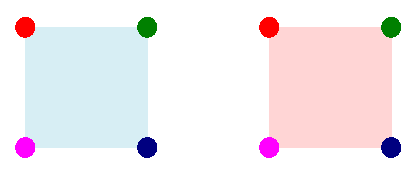
\includegraphics{figs/staggHypercubes.pdf}
  \caption{Example subdivision of one direction into disjoint hypercubes.
           Each hypercube is labeled by $h$, and the field $q(h)$
           associated to the hypercube is a linear combination of the
           $\chi$ fields on the corners, here represented by
           different colors. The effective lattice spacing between
           a $\chi$ of one corner of the blue hypercube and the corresponding
           $\chi$ in the same corner of the red hypercube is $a'=2a$.
           }
  \label{fig:staggHypercubes}
\end{figure}

We are now ready to carry out the substitution. The mass term follows
straightforwardly from the completeness relation. The kinetic term is
difficult, however, because the site offsets mix hypercubes. Therefore
it is crucially important to keep track of which hypercube $\chi$
belongs to. Keeping track of the hypercube will make manifest an $s$
dependence that makes applying the completeness relation not possible,
at least superficially. Gattringer and Lang~\cite{gattringer_quantum_2010}
suggest the following trick: we can shift the site that the first
hypercube starts on by one, which gives equivalent results as the
original hypercube labeling convention, and then average over these
two conventions. I wasn't able to figure this out. 
Rothe~\cite{rothe_lattice_2005} has another strategy, which I was also
not able to follow through. Nevertheless, one should find
\begin{equation}
S_F^{\rm stag}=a'^4\sum_h\Big(m\tr\left[\bar{q}q\right]
+\tr\left[\bar{q}\gamma_\mu\partial_\mu q\right]
-\frac{a'}{2}\tr\left[\bar{q}\gamma_5\Box_\mu q\gamma_\mu\gamma_5\right]\Big)
\end{equation}
where we have an implied summation over $\mu$, we have written
$q=q(h)$, introduced the effective spacing $a'\equiv2a$, and 
the discretized derivatives are
\begin{equation}
  \partial_\mu f(h)\equiv\frac{f(h+\hat{\mu})-f(h-\hat{\mu})}{2a'}
\end{equation}
and
\begin{equation}
  \Box_\mu f(h)\equiv\frac{f(h+\hat{\mu})-2f(h)+f(h-\hat{\mu})}{a'^2}.
\end{equation}

Our final step in the exploration of the staggered action will be to
identify the unphysical fermions. These {\it tastes} are hidden in
\index{taste}
the $q$. This should not be surprising because the $q_{ab}$ have 16
components, but Dirac spinors should have 4. This
tells us each $q$ corresponds to 4 spinors, and we will identify from
the $a$ and $b$ a taste index and Dirac index.
By comparing e.g. the $\tr[\bar{q}q]=\bar{q}_{ab}q_{ba}$ term with
what we expect from the physical, continuum theory, it makes sense
to identify the Dirac index with $b$. Thus our taste spinors are
\begin{equation}
  \psi^{t}(h)_\alpha\equiv q(h)_{\alpha t}~~~~\text{and}~~~~
  \bar{\psi}^{t}(h)_\alpha\equiv \bar{q}(h)_{t\alpha}.
\end{equation}
The staggered fermion action then becomes
\begin{equation}\label{eq:staggPhys}
S_F^{\rm stag}=a'^4\sum_h\left(
m\bar{\psi}^{t}\psi^{t}
+\bar{\psi}^{t}\gamma_\mu\partial_\mu\psi^{t}
-\frac{a'}{2}\bar{\psi}^{t}\gamma_5(\tau_5\tau_\mu)_{tt'}\Box_\mu\psi^{t'}
\right),
\end{equation}
where we have introduced new matrices
\begin{equation}
\tau_\mu\equiv\gamma_\mu^T.
\end{equation}

With the staggered action in the form of \equatref{eq:staggPhys} we can
begin to discuss some physics. The last term is called the
\index{taste!breaking}
{\it taste-breaking} term. It is similar to the Wilson term, in the
sense that it also represents a second derivative. However unlike
the Wilson term, it allows for interactions between fermions of
\index{taste!mixing}
different taste, i.e. it allows for {\it taste mixing}. If not for
the taste-breaking term, fermions of different taste would be mass-degenerate,
which one sees clearly from the first term. In the naive continuum limit,
this taste breaking terms vanishes like $a$.

The Wilson term broke axial symmetry completely, but in the taste-breaking
term, the remnant $\U_A(1)\times\U_A(1)$ remains. In particular this
term is invariant under transformations
\begin{equation}
\psi'=e^{i\omega}\psi, ~~~~~~
          \bar{\psi}'=\bar{\psi}e^{-i\omega}
\end{equation}
and
\begin{equation}
   \psi'=e^{i\omega\gamma_5\otimes\tau_5}\psi, ~~~~~~
          \bar{\psi}'=\bar{\psi}e^{i\omega\gamma_5\otimes\tau_5}.
\end{equation}
This latter symmetry follows from the fact that $\gamma_5$ commutes through
the taste-breaking term, while $\tau_5$ will pick up a minus sign.
One can identify this symmetry with a subgroup of the axial taste
symmetry group $\SU_A(N_t)$, where $N_t$ is the number of tastes.

At finite lattice spacing, taste mixing lifts the taste mass degeneracy.
One way to get some feeling for taste-breaking effects, then, is to look
at the mass spectrum of staggered fermions. It has been found that these
taste breaking effects can be reduced by improved gauge actions or smearing
\cite{durr_staggered_2004,follana_index_2004}, and in particular smearing
seems to drive masses to 4-fold degeneracy. An intuition for why smearing
might help is as follows: In the interacting theory, each $\chi$ is attached
to links according to its site, and since tastes are linear combinations
of these, it follows that different tastes touch different links. So
the more ``distance" in $\SU(N)$ space between the links, i.e. the more
the links fluctuate, the greater the taste-breaking effects will be.
Since smearing algorithms tend to drive links to more typical values
given their neighbors, they reduce these fluctuations, and hence
the taste-breaking.

We would also like to suppress the effects of unphysical tastes. Absent
taste-breaking, the Dirac operator corresponding to the staggered action
would be block diagonal in taste space, i.e. we would have for 
one physical flavor
\begin{equation}
D^{\rm stag}=\left(\begin{array}{cccc}
            D &   &  &  \\
              & D &  &  \\
              &   & D&  \\
              &   &  & D\\
            \end{array}\right).
\end{equation}
One commonly used strategy to remove the effects of taste-breaking is
\index{rooting}
therefore {\it rooting}. The idea is that $\det D^{\rm stag}$ is
the contribution to the probability distribution from four mass-degenerate
flavors. To isolate one of the flavors, it is sufficient to use
$\det D=(\det D^{\rm stag})^{1/4}$. For two degenerate light flavors
$m_l$ and one heavier flavor $m_s$, i.e. for $N_f=2+1$ fermions, 
one then samples with probability distribution
\begin{equation}\label{eq:HISQdist}
  \dd{\rm P}
    =\dd Ue^{-S_G}(\det D_l^{\rm stag})^{1/2}(\det D_s^{\rm stag})^{1/4}.
\end{equation}

In practice, taste-breaking is present at each lattice spacing, and
therefore it is not clear whether there is some leftover effect of rooting
in the continuum limit. In spite of this danger, people who employ staggered
actions often tend to use rooting anyway. One way to make this step more
justified is to reduce taste-breaking effects. Improved actions such
as the HISQ action, to be discussed in the next section, have greatly
reduced taste-breaking and, reassuringly, results from HISQ actions
seem to agree with experiment.

%\section{Questions}
%\begin{enumerate}
%  \item When can we find a power series expansion for a function of
%        Grassmann numbers?
%  \item Why do we want the integrand to vanish at the boundary?
%\end{enumerate}

\subsection{Highly improved staggered fermions}\label{sec:HISQ}
\index{action!HISQ}

Highly improved staggered quarks (HISQ) were introduced in 2007 by
Follana {\it et al.} \cite{follana_highly_2007}. This paper summarizes also
some of the history behind staggered quarks, and is written in a generally
friendly way; therefore I encourage the reader to have a look at it.

\index{taste!exchange}
Taste breaking can be thought of through {\it taste exchange}, where
one quark changes its taste by exchanging a virtual gluon with momentum
$p=\pi/a$; a quark with low enough momentum can thereby be pushed into
another corner of the Brillouin zone. See \figref{fig:treeLevelTasteExchange}
for a tree-level diagram.
\begin{figure}[t]
  \centering
  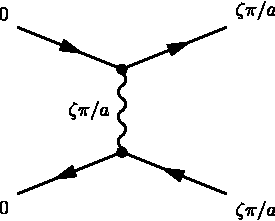
\includegraphics{figs/treelevel.pdf}
  \caption{A low-energy quark absorbing a gluon with momentum $\zeta\pi/a$
           can become a quark of another taste. Here $\zeta$ is a vector
           labelling some unphysical corner of the Brillouin zone. Image
           taken from Ref. \cite{follana_highly_2007}.
           }
  \label{fig:treeLevelTasteExchange}
\end{figure}
One goal of HISQ actions, then, is to suppress these processes, which is
done by smearing. Another way to look at taste violations is that they
are a lattice artifact, and so like any other lattice artifact, you would
like to remove its leading order contributions to improve the
approach to the continuum limit. Along this vein, another improvement
made by HISQ is to reduce lattice artifacts from the derivative discretization.

The basic strategy of HISQ can be summarized as:
\begin{enumerate}
  \item Improve finite difference derivatives by 
        \vspace{-1mm}
        \begin{equation*}
         \partial_\mu\to\partial_\mu-\frac{a^2}{6}(1+\epsilon)\partial_\mu^3,
        \end{equation*}
        where $\epsilon$ depends on charm physics. Without considering
        charm physics, this is called a {\it Naik term}.\index{Naik term}
  \item Find a smear $U_\mu\to\mathcal{F}_\mu U_\mu$ that vanishes
        for links carrying momentum $\pi/a$. We start with one
        called {\it Fat7}.\index{Fat7 link}
  \item Multiple smearing reduces mass splittings more, so do that.
  \item Remove new $\mathcal{O}(a^2)$ errors introduced by Fat7.
  \item Smearing enhances some one-loop taste exchange processes,
        which can be suppressed by reunitarizing.
\end{enumerate}
Overall the HISQ smear is then
\begin{equation}\label{eq:HISQsmear}
\mathcal{F}^{\rm HISQ}\equiv
\mathcal{F}^{\rm Fat7}_{\rm corr}\mathcal{U}\mathcal{F}^{\rm Fat7},
\end{equation}
where $\mathcal{F}^{\rm Fat7}_{\rm corr}$ has been corrected for the
errors referenced in step 4, and $\mathcal{U}$ is the reunitarization
operator needed for step 5. The HISQ action uses link variables smeared
by \equatref{eq:HISQsmear}, and its kinetic term uses improved
Naik discretization.

To judge how well the HISQ action does, the authors of
Ref.~\cite{follana_highly_2007} calculated several one-loop taste
exchange processes (that fall into several broad categories indicated
in \figref{fig:oneLoopTasteExchange}) and determined their coefficients, 
$d$. \tabref{tab:hisq} compares the suppression of taste exchange
to other smearing programs. Before HISQ, ASQTAD was a popular dynamical
fermion action, and one sees that, measured in this way, taste effects
in the HISQ action are reduced by an order of magnitude.
\begin{figure}[t]
  \centering
  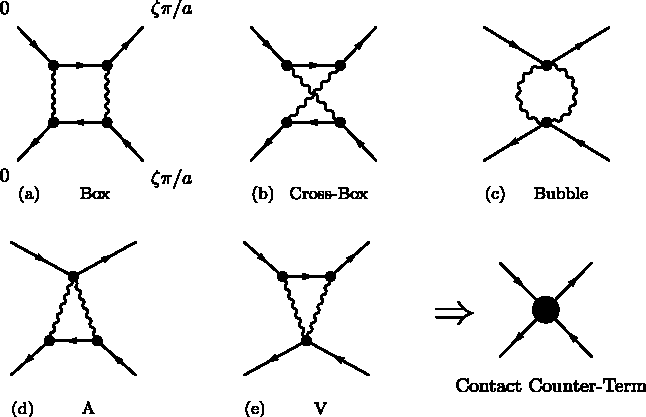
\includegraphics{figs/oneloop.pdf}
  \caption{Some example one-loop processes contributing to taste exchange.
           Image taken from Ref. \cite{follana_highly_2007}.
           }
  \label{fig:oneLoopTasteExchange}
\end{figure}
\begin{table}[t]
\begin{tabularx}{\linewidth}{lCCCC} \hline\hline
        & \multicolumn{3}{c}{Unimproved} & Improved \\
         & ASQTAD & HISQ & HYP & ASQTAD \\ \hline
         Avg $d$,$\tilde{d}$ & 0.23 & 0.02 & 0.02 & 0.13\\
        \hline\hline 
\end{tabularx}
\caption{Average coefficients for the taste processes indicated
         in \figref{fig:oneLoopTasteExchange} for a few
         types of lattice actions. Columns indicate whether the
         gluons are improved. Excerpt from Table II of
         Ref. \cite{follana_highly_2007}.}
\label{tab:hisq}
\end{table}

%\section{Overlap fermions}

\section{Improved actions and interpolators}

In LFT the correlation length $\xi$ is related to the mass $m$ of the lightest 
\index{correlation length}\index{improvement}
particle by
\begin{equation}
  \xi=\frac{1}{ma}.
\end{equation}
This can be seen from looking at the spectral decomposition of the
connected correlation function
\begin{equation}\label{eq:spectralDecomp}
  \ev{X(x)X(y)}_c=\sum_{n> 0} 
                   \left|\bra{0}X\ket{n}\right|^2
                    e^{-(E_n-E_0)\Delta t},
\end{equation}
which has been evaluated at $\vec{x}=\vec{y}=0$ for notational simplicity and
we define $\Delta t$ as the temporal distance between $x$ and $y$.
For large $\Delta t$ we find schematically
\begin{equation}
  \ev{X(x)X(y)}_c\sim e^{(E_1-E_0)\Delta t} =e^{-m\Delta t}=e^{-\Delta t/\xi}.
\end{equation}

Equation~\eqref{eq:spectralDecomp} measures how correlated the field 
$X$ at $x$ is with the field at $y$. In the continuum limit, $\xi$ will 
diverge since $m$ is constant, i.e. the system experiences a second-order 
phase transition. Correspondingly the correlation function increases to
maximum correlation. The divergence of $\xi$ implies a divergence in the
integrated autocorrelation time
\index{critical slowing down}\index{critical exponent!dynamical}
\begin{equation}\label{eq:criticalSlowingDown}
  \tau_{\text{int}, X} \sim \xi_X^z
\end{equation}
with {\it dynamical critical exponent} $z$ that depends on the algorithm 
details. For $z\neq 0$, \equatref{eq:criticalSlowingDown} implies a
deterioration in the efficacy of the updating process toward the
continuum limit; this is {\it critical slowing down}.

Due to critical slowing down, configuration generation becomes increasingly
expensive as one lowers the lattice spacing.
On the other hand, one wishes to minimize discretization error. One way to
proceed is as follows: There are multiple discretizations of a lattice action
that will lead to the same continuum limit action, so one can design a lattice
action where one suppresses the discretization effects by hand. Such actions
are examples of {\it improved actions}. They are in general slower to generate
configurations at a given $a$ than unimproved actions, but have the advantage
of being in some sense ``closer to the continuum limit" than the unimproved
actions at a given $N_\tau$.

One knows that the Wilson action has
$\order{a^2}$ discretization errors. If we add to the Wilson action some
$\order{a^2}$ terms out, we will have eliminated all discretization error
up to $\order{a^3}$. This is called an $\order{a^3}$ {\it improved action}
or an $\order{a^4}$ {\it action}. Ultimately, our goal is to calculate
expectation values, so we will generally also want to improve our 
lattice interpolators. 
%For instance suppose we find some $\order{a^p}$
%action $S_\text{lat}$ with $p\geq1$. Generically it is related to the 
%continuum action $S_{\text{cont}}$ by
%\begin{equation}
%  S_\text{lat}=S_\text{cont}+a^pS_p+\order{a^{p+1}},
%\end{equation}
%where $S_p$ is a correction term with dimension [fm$^{-p}$]. (Since masses are
%inverse lengths, this is often called {\it mass dimension}.) 
%\index{mass dimension} Similarly we will
%have for our interpolator $X_\text{lat}$ 
%\begin{equation}
%   X_\text{lat} = X_\text{cont}+a^qX_q +\order{a^{q+1}}
%\end{equation}
%with $q\geq1$. Expanding the exponential, one finds for the partition function
%\begin{equation}
%  Z_\text{lat}=Z_\text{cont}\left(1-a^p\ev{S_p}+\order{a^{p+1}}\right),
%\end{equation}
%from which it follows that
%\begin{equation}
%\ev{X_\text{lat}}=\ev{X_\text{cont}}+\order{a^p,a^q},
%\end{equation}
%i.e. the discretization error in the expectation value is controlled by both
%the action and the interpolator, whichever is worse.

In what follows, we will look at some improvement strategies, guided by 
Chapter 10 of \cite{degrand_lattice_2006} and Chapter 9 of
\cite{gattringer_quantum_2010}, where there is also more discussion to 
be found. Improvement schemes are rather technically
involved, so I will not be able to verify all details carefully.

\subsection{Symanzik improvement}\label{sec:symanzikImprovement}

The Symanzik improvement scheme \cite{symanzik_continuum_1983,
symanzik_continuum_1983-1,curci_symanziks_1983,luscher_shell_1985} 
is a systematic way to\index{improvement!Symanzik}
improve lattices actions. Gattringer and Lang summarize the strategy as
carrying out the following steps:
\begin{enumerate}
  \item Start with a discretized version of your quantity $Q$.
  \item Identify correction terms using the continuum theory, keeping in mind
        what it allowed given the symmetries of $Q$, and organize them according
        to their mass dimension.
  \item Add discretized versions of the correction terms, multiplied with
        suitable coefficients, to the discretized version of $Q$ so that 
        lattice artifacts vanish up to the desired order.
\end{enumerate}
There is often more than one way to pick correction terms.

We begin by improving the gauge action. In the continuum theory, the gauge
action is proportional to the dimension-four operator
\begin{equation}
  O_4 = \tr F_{\mu\nu}F_{\mu\nu}.
\end{equation}
Our first correction term is at $\order{a^2}$, and there are no dimension-five
operators anyway, so we write the three dimension-six operators\footnote{You 
can convince yourself this is all there is by keeping track of the
dimensions of the comprising operators, for example $D_\mu$ has mass dimension
one and $F_{\mu\nu}$ therefore has mass dimension two, and by demanding gauge
and Lorentz invariance. In the end you need two $D_\mu$'s and two 
$F_{\mu\nu}$'s, and there are three different ways to contract their 
Lorentz indices.}
\begin{equation}\begin{aligned}
  O_{6a}&=\sum_{\mu\nu}\tr D_\mu F_{\mu\nu} D_\mu F_{\mu\nu},\\
  O_{6b}&=\sum_{\mu\nu\rho}\tr D_\mu F_{\nu\rho} D_\mu F_{\nu\rho},\\
  O_{6c}&=\sum_{\mu\nu\rho}\tr D_\mu F_{\mu\rho} D_\nu F_{\nu\rho}.
\end{aligned}\end{equation}
If we expand the plaquette in the lattice spacing, all of the above
operators will appear:
\begin{equation}
  \tr \plaq = N_c + \frac{1}{2}a^4O_4+a^6\sum_i r_iO_{6i},
\end{equation}
where $i\in\{\text{a, b, c}\}$.

\begin{figure}
  \centering
  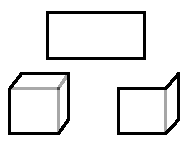
\includegraphics[width=0.5\linewidth]{figs/luescherWeisz.pdf}
  \caption{Lattice dimension-six operators. The top is the rectangle, the
           bottom-left is the parallelogram, and the bottom-right is the 
           chair. Light grey lines are to guide the eye.}
  \label{fig:dim6operators}
\end{figure}
To improve our gauge action thus requires at least three dimension-six
lattice operators. The simplest are the rectangle ``rt", the parallelogram
``pg", and the chair ``ch", which are depicted in 
\figref{fig:dim6operators}. Their multiplicities are listed in
\tabref{tab:dim6operators}. An improvement on the Wilson action could
then be written as
\begin{equation}
  S_\text{LW}=\frac{\beta}{3}\sum_i c_i \Re\tr\left(\id-U_i\right),
\end{equation}
where $i\in\{\text{pl, rt, pg, ch}\}$, with ``pl" standing for plaquette,
and $U_i$ is the corresponding lattice operator. In their original paper,
L\"uscher and Weisz chose the normalization
\begin{equation}\label{eq:LWnorm}
  c_\text{pl}+8c_\text{rt}+8c_\text{pg}+16c_\text{ch}=1.
\end{equation}

\begin{table}
\begin{tabularx}{\linewidth}{LR} \hline\hline
         Operator type & Number elements per site\\\hline
         Rectangle & 12 \\
         Parallelogram & 16 \\
         Chair & 48\\
        \hline\hline 
\end{tabularx}
\caption{Dimension-six operator multiplicities. Loops that differ by
         orientation only are considered equal.}
\label{tab:dim6operators}
\end{table}

To fix the coefficients, one chooses an improvement condition, for example
that the zero-temperature static potential gives
\begin{equation}
  V(r)\approx\frac{1}{r}
\end{equation}
up to $\order{a^4,g^2a^2}$. This yields 
\begin{equation}
  c_\text{pg}=0~~~~\text{and}~~~~c_\text{rt}+c_\text{ch}=-\frac{1}{12}.
\end{equation}
Furthermore since there are the most chair operators, it is convenient
to pick $c_\text{ch}=0$. According to the normalization condition
\equatref{eq:LWnorm}, one thus finds
\begin{equation}
  c_\text{pl}=\frac{5}{3},~~~~c_\text{rt}=-\frac{1}{12},~~~~
    c_\text{pg}=c_\text{ch}=0,
\end{equation}
which is called the {\it L\"uscher-Weisz} action~\cite{luscher_shell_1985}.
\index{action!L\"uscher-Weisz}

Next we turn to an improvement of the Wilson fermionic action. Now the leading
correction is $\order{a}$, and owing to $\bar{\psi}\psi$ being dimension-three,
there is now the possibility for dimension-five operators. Demanding that
our operators satisfy the symmetries of the Wilson action, e.g.
charge conjugation $\qconj$ and parity $\parity$, we end up in the
continuum with 
\begin{equation}\begin{aligned}
  O_{5a}&=\bar\psi \sigma_{\mu\nu}F_{\mu\nu}\psi, \\
  O_{5b}&=\bar\psi\left(\Dright_\mu\Dright_\mu
                          +\Dleft_\mu\Dleft_\mu\right)\psi,\\ 
  O_{5c}&=m \tr F_{\mu\nu}F_{\mu\nu},\\
  O_{5d}&=m\bar\psi\left(\overrightarrow{\slashed{D}\strut}
                         -\overleftarrow{\slashed{D}\strut}\right)\psi,\\
  O_{5e}&=m^2 \bar\psi \psi,
\end{aligned}\end{equation}
where
\begin{equation}
  \sigma_{\mu\nu}\equiv\frac{1}{2i}[\gamma_\mu,\gamma_\nu].
\end{equation}
This list of operators can be reduced by using the field equation
\begin{equation}
 (\slashed{D}+m)\psi=0,
\end{equation}
from which it follows
\begin{equation}
  O_{5a}-O_{5b}+2O_{5e}=0~~~~\text{and}~~~~O_{5d}+2O_{5e}=0,
\end{equation}
i.e. $O_{5b}$ and $O_{5d}$ are linearly dependent on the other operators,
and can therefore be eliminated. Of the remaining operators, $O_{5c}$ and
$O_{5e}$ are, up to the factor $m$, present in the original action, so
they can be absorbed in the original action by redefining the bare
parameters $m$ and $g$.

\begin{figure}
  \centering
  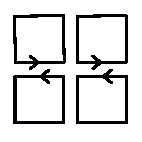
\includegraphics[width=0.5\linewidth]{figs/clover.pdf}
  \caption{The ``clover" sum $Q_{\mu\nu}(x)$ used in the discretization of the
           field strength $\hat{F}_{\mu\nu}$ in \equatref{eq:cloverField}.
           The point $x$ is in the middle of the squares.}
           
  \label{fig:clover}
\end{figure}

Taken altogether, all that remains for improvement is the operator $O_{5a}$,
so that the $\order{a}$ improved Wilson fermion action becomes
\begin{equation}\label{eq:cloverAction}
  S_\text{clover}=S_\text{Wilson}+\frac{c_\text{SW}}{2}
               \,a^5\sum_{x;\,\mu<\nu}\bar{\psi}(x)
                  \sigma_{\mu\nu}\hat{F}_{\mu\nu}\psi(x),
\end{equation}
with the real {\it Sheikholeslami-Wohlert} coefficient $c_\text{SW}$
\cite{sheikholeslami_improved_1985} and $\hat{F}_{\mu\nu}$ being the
\index{Sheikholeslami-Wohlert}
following discretization of the field strength tensor:
\begin{equation}\label{eq:cloverField}
  \hat{F}_{\mu\nu}(x)\equiv
    -\frac{i}{8a^2}\left(Q_{\mu\nu}(x)-Q_{\nu\mu}(x)\right)
\end{equation}
where $Q_{\mu\nu}(x)$ is the plaquette sum (see \figref{fig:clover})
\begin{equation}
  Q_{\mu\nu}(x)\equiv U_{\mu\nu}(x)+U_{\nu,-\mu}(x)
                 +U_{-\mu,-\nu}(x)+U_{-\nu,\mu}(x).
\end{equation}
Due to the shape of $Q_{\mu\nu}$, the latter term in 
\equatref{eq:cloverAction} is called the {\it clover term}, and the
action is said to be {\it clover-improved}.\index{action!clover-improved}
This discretization of $F_{\mu\nu}$ is chosen because it is more
symmetric than the simple plaquette discretization.
The coefficient $c_\text{SW}$ can be calculated perturbatively; one finds
\cite{sheikholeslami_improved_1985}
\begin{equation}\label{eq:SWcoeff}
  c_\text{SW}=1+0.2659 g^2+\order{g^4}.
\end{equation} 

To round out our discussion of Symanzik improvement, we now turn to the
improvement of some interpolators. The hitherto discussed action improvements
suffice to improve on-shell quantities, e.g. hadron masses, at $\order{a}$. 
For these on-shell quantities, only eigenstates of the Hamiltonian
contribute. However it is not enough for off-shell quantities such as
correlators, which have off-diagonal contributions, and their interpolators
need to be improved. We will discuss now two examples, the isovector axial
current $A_\mu^a$ and the pseudoscalar density $P^a$,
\begin{equation}\begin{aligned}
A_\mu^a&=\frac{1}{2}\bar{\psi}\gamma_\mu\gamma_5\sigma^a\psi,\\
P^a&=\frac{1}{2}\bar{\psi}\gamma_5\sigma^a\psi.
\end{aligned}\end{equation}
The dimension-four operators needed to improve $A_\mu^a$ are
\begin{equation}\begin{aligned}
  O_{4a,\mu}^a&=\frac{1}{2}\bar{\psi}\gamma_5\sigma_{\mu\nu}
                 \left(\Dright_\nu-\Dleft_\nu\right)\sigma^a\psi,\\
  O_{4b,\mu}^a&=\frac{1}{2}\partial_\mu
                  \left(\bar{\psi}\gamma_5\sigma^a\psi\right)\\
  O_{4c,\mu}^a&=\frac{m}{2}\bar{\psi}\gamma_\mu\gamma_5\sigma^a\psi.
\end{aligned}\end{equation}
Again, as before, we can apply the Dirac equation to show $O_{4a,\mu}$ is
linearly dependent on the other two, and again $O_{4c,\mu}$ is equal to
the original current up to the factor $m$, so it can be absorbed
in a redefinition. The improved current is therefore
\begin{equation}
  A_{\text{imp},\mu}^a=A_\mu^a+c_A a\hat{\partial}_\mu P^a,
\end{equation}
where $c_A\in\R$ and $\hat{\partial}$ is the symmetric difference
discretization of the derivative. From perturbation theory one finds
\begin{equation}
  c_A=-0.00756g^2+\order{g^4}.
\end{equation}
With this discussion we see that the
operator $O_{4c,\mu}$ can be absorbed into a redefinition of $P^a$, i.e.
\begin{equation}
  P_\text{imp}^a=P^a.
\end{equation}

\subsection{Tadpole improvement}\index{improvement!tadpole}

\begin{figure}
  \centering
  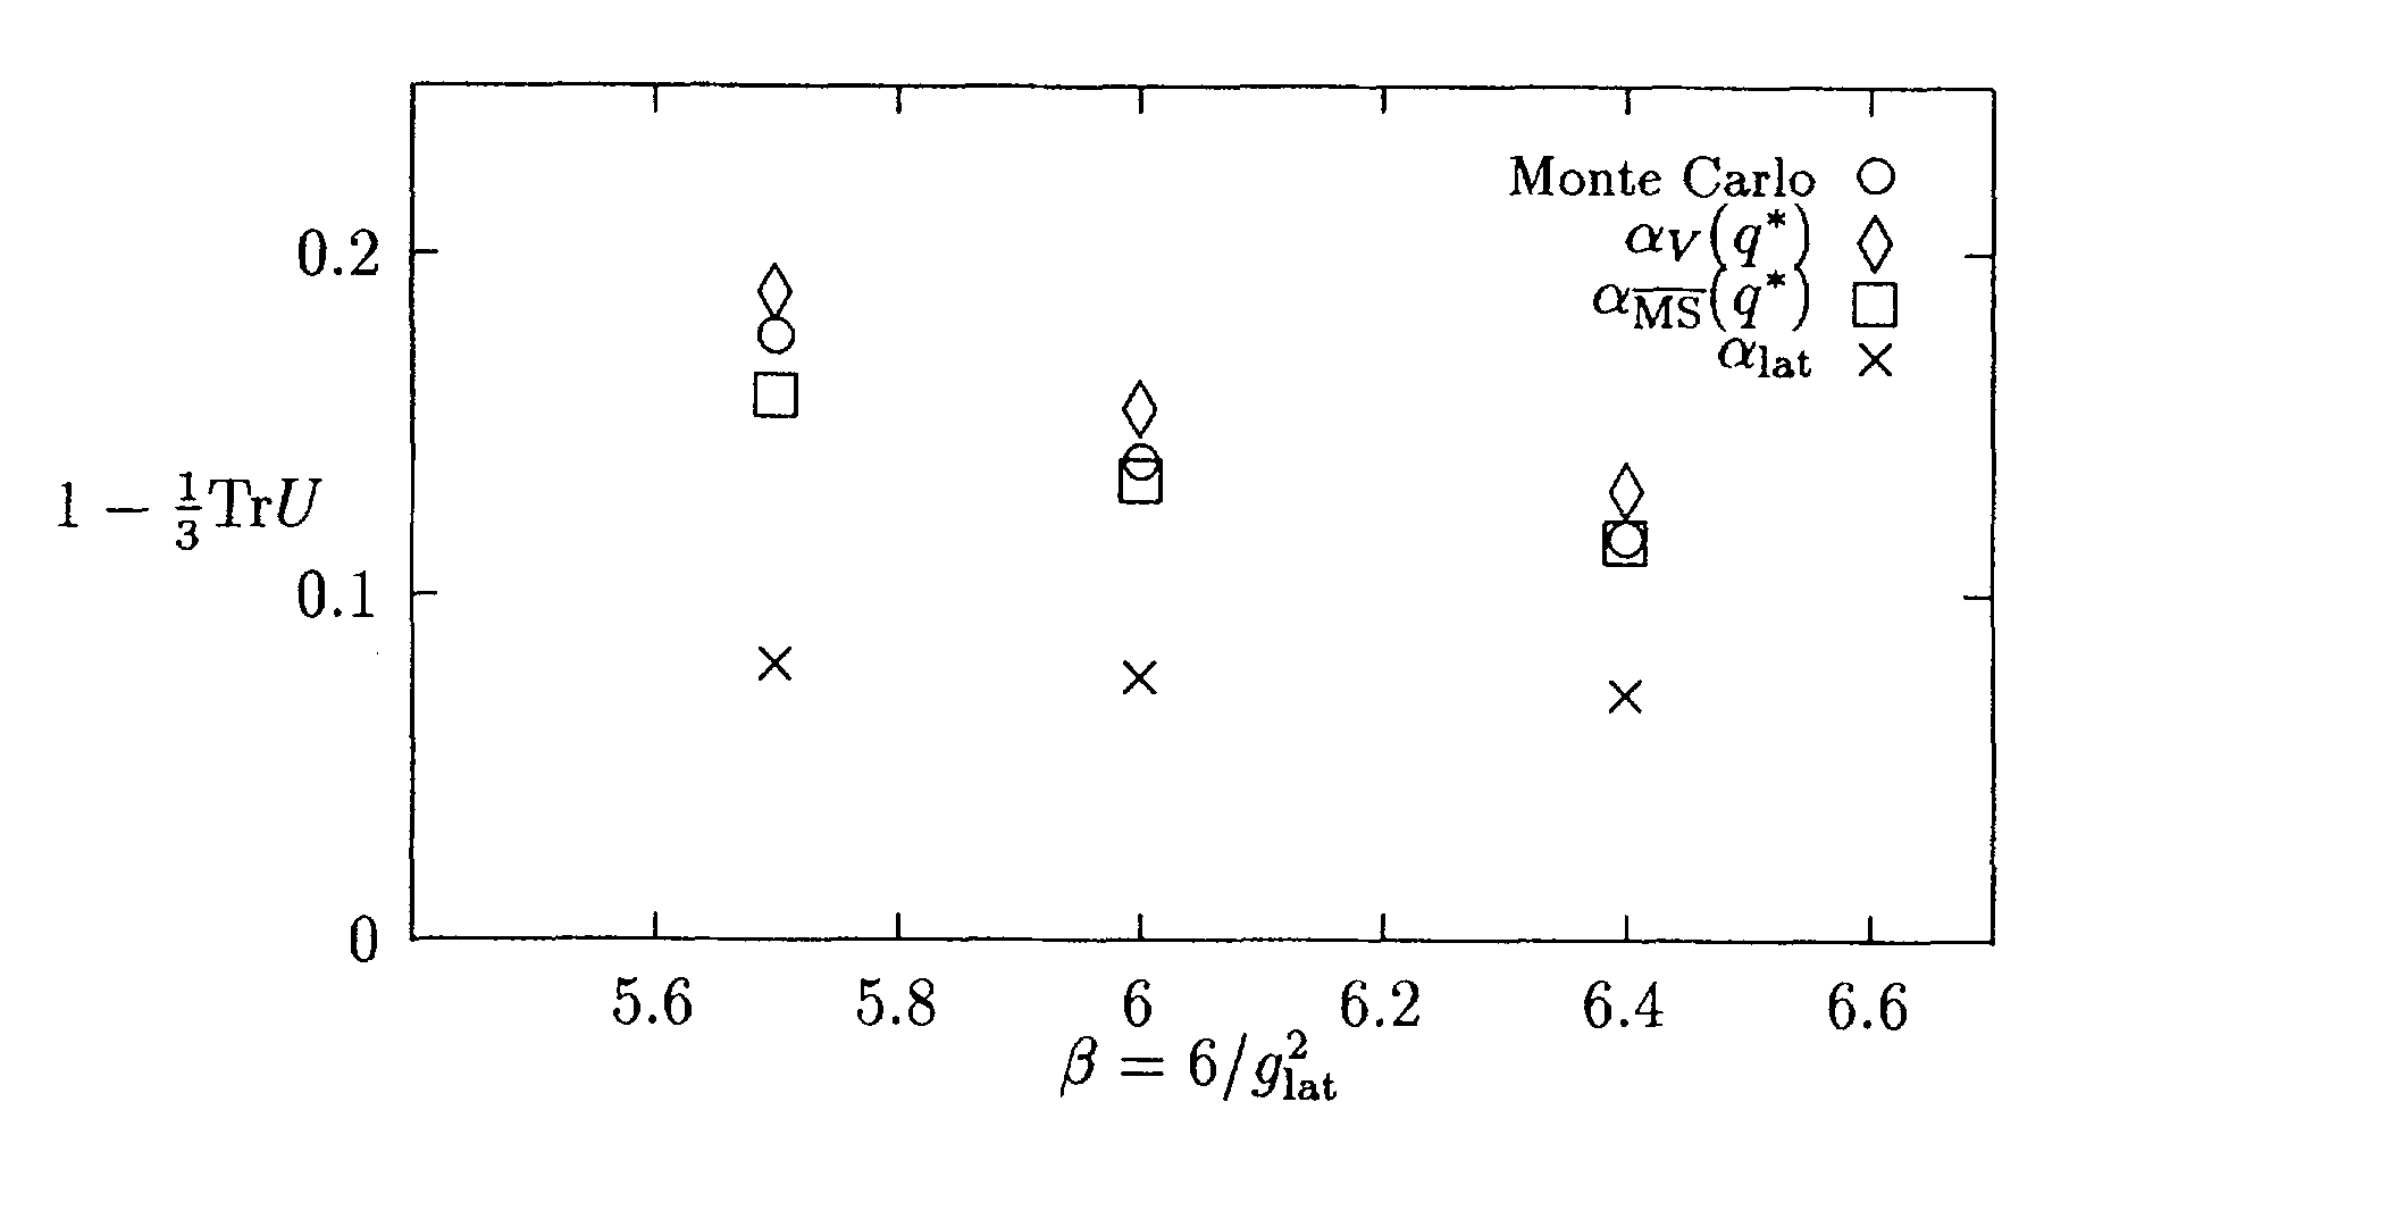
\includegraphics[width=\linewidth]{figs/averageLink.png}
  \caption{Expectation value of the trace of a link, evaluated in the
           Landau gauge. Results are calculated by MCMC and in first-order
           perturbation theory, expanding in two ``good" parameters
           (see Ref.~\cite{lepage_viability_1993}) and the lattice
           coupling. These were carried out for quenched configurations
           with $\beta\geq5.7$. Image taken from 
           Ref.~\cite{lepage_viability_1993}.}
  \label{fig:averageLink}
\end{figure}

In the early 1990's, physicists working in lattice field theory encountered
a somewhat troubling problem: Many quantities calculated perturbatively
in the bare coupling constant $g\equiv g_\text{lat}$ turned out to differ
substantially from MCMC results, even for rather small lattice spacing.
An example of the failure was calculated by Lepage and Mackenzie
\cite{lepage_viability_1993}, and is shown in \figref{fig:averageLink}.
In this paper, the authors argue that $g_\text{lat}$ is a poor expansion
parameter, and they give two alternative couplings that converge better.

\begin{figure}
  \centering
  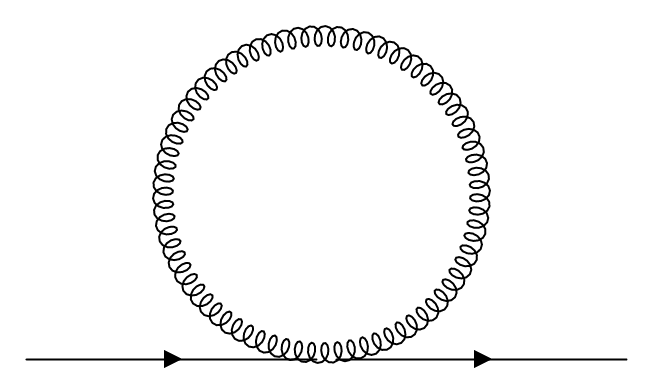
\includegraphics[width=0.5\linewidth]{figs/tadpole.png}
  \caption{A tadpole diagram contributing to the fermion self-energy.}
  \label{fig:tadpole}
\end{figure}

More pertinent to this discussion of action and interpolator improvement
is the origin of this mismatch, which they also investigate. They argue as
follows: In lattice perturbation theory one can expand the link variable as
\begin{equation}
  U_\mu(x)=\exp\left[igaA_\mu^a(x)T^a\right]
          =\id+iagA_\mu^a(x)+\order{a^2g^2}.
\end{equation}
Superficially it seems as though we always get some power of $ag$, but for
tadpole diagrams, their divergence in $a$ exactly cancels the power of $a$ 
coming from the vertex. These diagrams therefore are suppressed by a
power of $g$ only. An example tadpole is shown in \figref{fig:tadpole}.
These tadpoles come from the UV part of loop integrals. To obtain a
better behaved perturbative expansion, one could imagine factoring out
(integrating out) this UV contribution, so that the perturbative expansion
would instead read
\begin{equation}
  U_\mu(x)\approx u_0\left(\id+iagA^{\text{IR},a}_\mu(x)T^a\right),
\end{equation}
with the {\it tadpole factor} $u_0$ and with the gauge field only 
including\index{tadpole factor}
IR modes. Here $u_0$ has to be a constant\footnote{Otherwise we are not
guaranteed that $U_\mu(x)$ will work correctly as a gauge connection.}, 
and it represents the average value of the link.

In \secref{sec:symanzikImprovement}, improvement coefficients were
determined using perturbation theory. One can imagine that our coefficients
will be better determined taking the influence of tadpoles into account.
This is called {\it tadpole improvement}, and to employ it, we need to
determine $u_0$\footnote{In general $u_0$ depends on the parameters of the
theory.}. One could imagine extracting it from the average link; to do
this one must fix to a particular gauge, since a single link is a
gauge-dependent quantity that would therefore otherwise vanish. One
can also measure it from gauge-invariant constructions such as
\begin{equation}
  u_0=\left(\frac{1}{N_c}\ev{\tr \plaq}\right)^{1/4}.
\end{equation}
Tadpole improvement then amounts to replacing all links $U_\mu$ in lattice
expressions with $U_\mu/u_0$.

As a simple example we present the tree-level, tadpole-improved, one-flavor
clover Lagrangian density. We rescale the action by multiplying by 
the hopping parameter
\begin{equation}
  2\kappa=\frac{1}{m+4/a},
\end{equation}
rescaling the fermion fields by the factor $\sqrt{m+4/a}$, and
rescaling the link variables by the tadpole factor to get
\begin{equation}\begin{aligned}
  \Lagr_\text{clover}^\text{tad}=~&\bar{\psi}(x)\psi(x)\\
    &-\frac{\kappa}{u_0}\frac{1}{a}\bar{\psi}(x)
    \sum_{\mu=\pm1}^{\pm4}\left(\id-\gamma_\mu\right)U_\mu(x)
           \delta(x+a\hat{\mu}-y)\,\psi(y)\\
    &+\,\frac{\kappa}{u_0}\frac{c_\text{SW}}{u_0^3}
               \,a^5\sum_{\mu<\nu}\bar{\psi}(x)
                  \sigma_{\mu\nu}\hat{F}_{\mu\nu}\psi(x).
\end{aligned}\end{equation}
Using this Lagrangian in a simulation is exactly like using the original 
clover Lagrangian in a simulation; one just has a new hopping parameter
$\kappa'=\kappa/u_0$. From \equatref{eq:SWcoeff}, one finds the
tree-level, tadpole-improved Sheikholeslami-Wohlert coefficient to be
simply
\begin{equation}
  c_{SW}=\frac{1}{u_0^3}.
\end{equation}
One can improve beyond tree-level; for details I refer the reader
to Ref.~\cite{degrand_lattice_2006}.

\subsection{Fat links}\index{fat link}

Typically the gauge connection between two neighboring sites $x$ and $y$
on the lattice is just a single link $U(x,y)$, which is in some sense the 
most local connection imaginable. One can also relax this locality, so that 
the gauge connection contains information from a larger region around 
$x$ and $y$; for example the connection could depend on a general sum, 
including many paths connecting $x$ and $y$. Let's call
this sum $\Sigma(x,y)$. Then the gauge connection could be $V(x,y)$,
where $V$ is chosen by extremizing $\tr V\Sigma^\dagger$. These gauge
connections are called {\it fat links} \cite{blum_improving_1997}. 
We encountered fat links
already in \secref{sec:HISQ}, where they were employed to reduce
taste-breaking effects, and indeed one of the reasons to use a fat link
is to correct hadron spectra. It should not surprise you that fat links
modify particle spectra, since they amount to a change of the lattice 
propagator.

Replacing a link by some weighted sum connecting $x$ and $y$ is consistent
with gauge invariance and hypercube symmetries of the lattice. These are
smeared gauge links. Replacing a link by a weighted average that is displaced
in directions perpendicular to the direction of the connection is a
discretization of higher order derivatives $\partial^2_\nu A_\mu$
\cite{blum_improving_1997} with $\mu\neq\nu$. For example the use of a
fat link might amount to a change
\begin{equation}
  U_\mu\to \left[1+\frac{\epsilon a^2 \Delta^2}{n}\right]^n U_\mu,
\end{equation} 
where $n$ is a small integer and $\epsilon$ is a smearing parameter
\cite{lepage:1997id}. This changes the gluon propagator by a factor
$\exp[-\epsilon a^2q^2]$ in momentum space, i.e. UV modes are 
significantly attenuated. One then sees a connection to Symanzik improvement:
By choosing $\epsilon$ carefully, one can adjust, e.g., 
$\order{a^2}$ corrections.

\begin{figure}
  \centering
  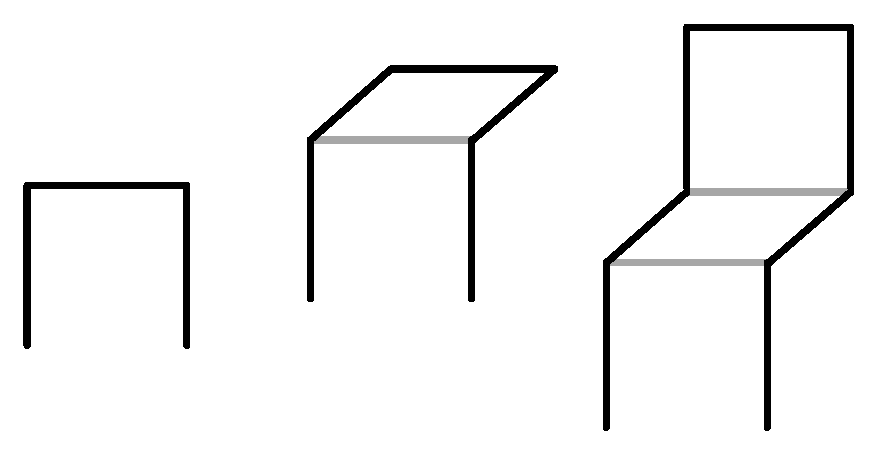
\includegraphics[width=0.6\linewidth]{figs/linkConstructs.pdf}
  \caption{Example three-link, five-link, and seven-link constructs that
           go into the AsqTad fat links. Light grey lines guide the eye.}
  \label{fig:AsqTadConstructs}
\end{figure}

Here we present the AsqTad\index{action!AsqTad}
action~\cite{orginos_variants_1999,lepage_flavor-symmetry_1999}, a staggered
fermion action with nearest- and third-nearest-neighbor interactions
\begin{equation}
  \Delta_\mu-\frac{a^2}{6}\Delta_\mu^3,
\end{equation}
i.e. it uses the Naik term.
The third-nearest-neighbor uses an ordinary link, but the nearest-neighbor
uses the fat link
\begin{equation}
  V_\mu=~c_1U_\mu
           +\sum_\nu\left[w_3S_{\mu\nu}^{(3)}
           +\sum_\rho\left(w_5S_{\mu\nu\rho}^{(5)}
           +\sum_\sigma w_7S^{(7)}_{\mu\nu\rho\sigma}\right)
            +w_LS^{(L)}_{\mu\nu}\right],
\end{equation}
where the link constructs are given by
\begin{equation}\begin{aligned}
  S_{\mu\nu}^{(3)}(x)
       &=U_\nu(x)U_\mu(x+a\hat{\nu})U_\nu^\dagger(x+a\hat{\mu}),\\
  S_{\mu\nu\rho}^{(5)}(x)
       &=U_\nu(x)S_{\mu\rho}^{(3)}(x+a\hat{\nu})U_\nu^\dagger(x+a\hat{\mu}),\\
  S_{\mu\nu\rho\sigma}^{(7)}(x)
       &=U_\nu(x)S_{\mu\rho\sigma}^{(5)}(x+a\hat{\nu})
         U_\nu^\dagger(x+a\hat{\mu}),\\
  S_{\mu\nu}^{(L)}(x)
       &=U_\nu(x)S_{\mu\nu}^{(3)}(x+a\hat{\nu})U_\nu^\dagger(x+a\hat{\mu}).
\end{aligned}\end{equation}
Examples of these constructs are shown in \figref{fig:AsqTadConstructs}.
The tadpole-improved coefficients are
\begin{equation}
  c_1=8w_5=48w_7=\frac{1}{8}w_L=-\frac{1}{16}~~~~~~\text{and}~~~~~~
     w_3=-\frac{5}{16}.
\end{equation}


\bibliographystyle{unsrtnat}
\bibliography{bibliography}
